\section{Regular Integral in 2D}

\subsection*{1 Dimensional Integration}

In 1 dimensional integration, we have a function that depends only on $x$. We can plot the function in 2D, by letting the $y = f(x)$. This is called the graph of the function.

When we integrate a function, the domain of integration needs to be an interval $[a, b]$. The interval can be interpreted as a 1 dimensional object. \bred{The dimension of the domain must match the dimension of the function}.

The result of the integral represents the (2 dimensional) area under the curve $y = f(x)$ above the interval $[a, b]$ (if $f(x) > 0$).

\subsection*{2 Dimensional Integration}

In 2 dimensional integration, we have a function that depends on $x$ and $y$. For example, $f(x, y) = xy + x^2$ or $f(x, y) = e x \sin(xy + 1)$. 

Similar to the case that $f(x) = 10$ can be considered as a 1D function, $f(x, y) = 2x$, $f(x, y) = e^y$ or $f(x, y) = 5$, can all be considered as a 2D function, even though they may only depend on one or none of the variables.

If we were to calculate the 2D integral of these functions by considering them as 2D functions, the answer would be different than their 1D integral (where we consider them as 1D functions).

To plot a 2D function, we can let $z = f(x, y)$. The value of the function will be the height of the point plotted in 3D space. This is the graph of a 2D function. It will be a 2D surface in 3D.

% TODO: graph of z = sin(y) + 2x
\begin{center} 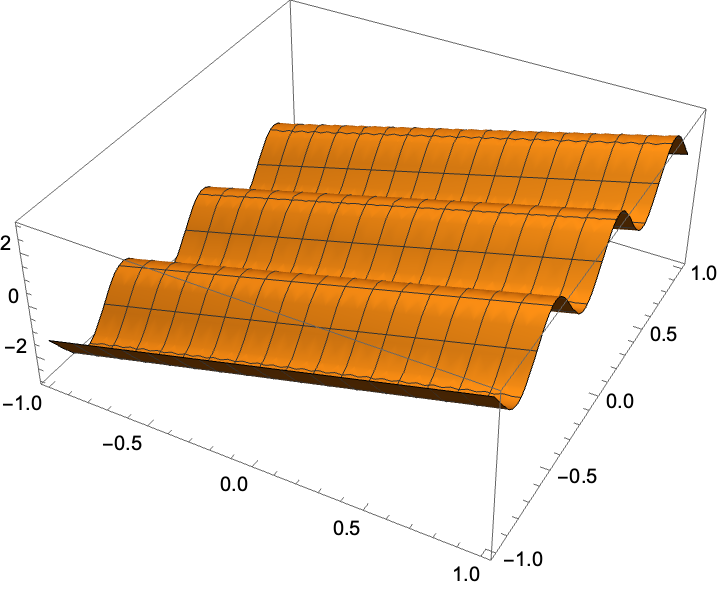
\includegraphics[width=0.275\linewidth]{Plots/s_4_1/sin(y)+2x.png} \end{center}

When we integrate a 2D function $f(x, y)$, the domain of integration needs to be a patch of area on the $xy$-plane. Perhaps the domain is a square, or a circle, or some area that is irregularly shaped. Regardless, the domain must be a \bred{2 dimensional object} on the $xy$-plane. \bred{The dimension of the domain must match the dimension of the function}.

The value of the integral over the domain corresponds to the \bred{3D volume} under the curved surface $f(x, y)$ \bred{above the domain of integration}.

\begin{center} 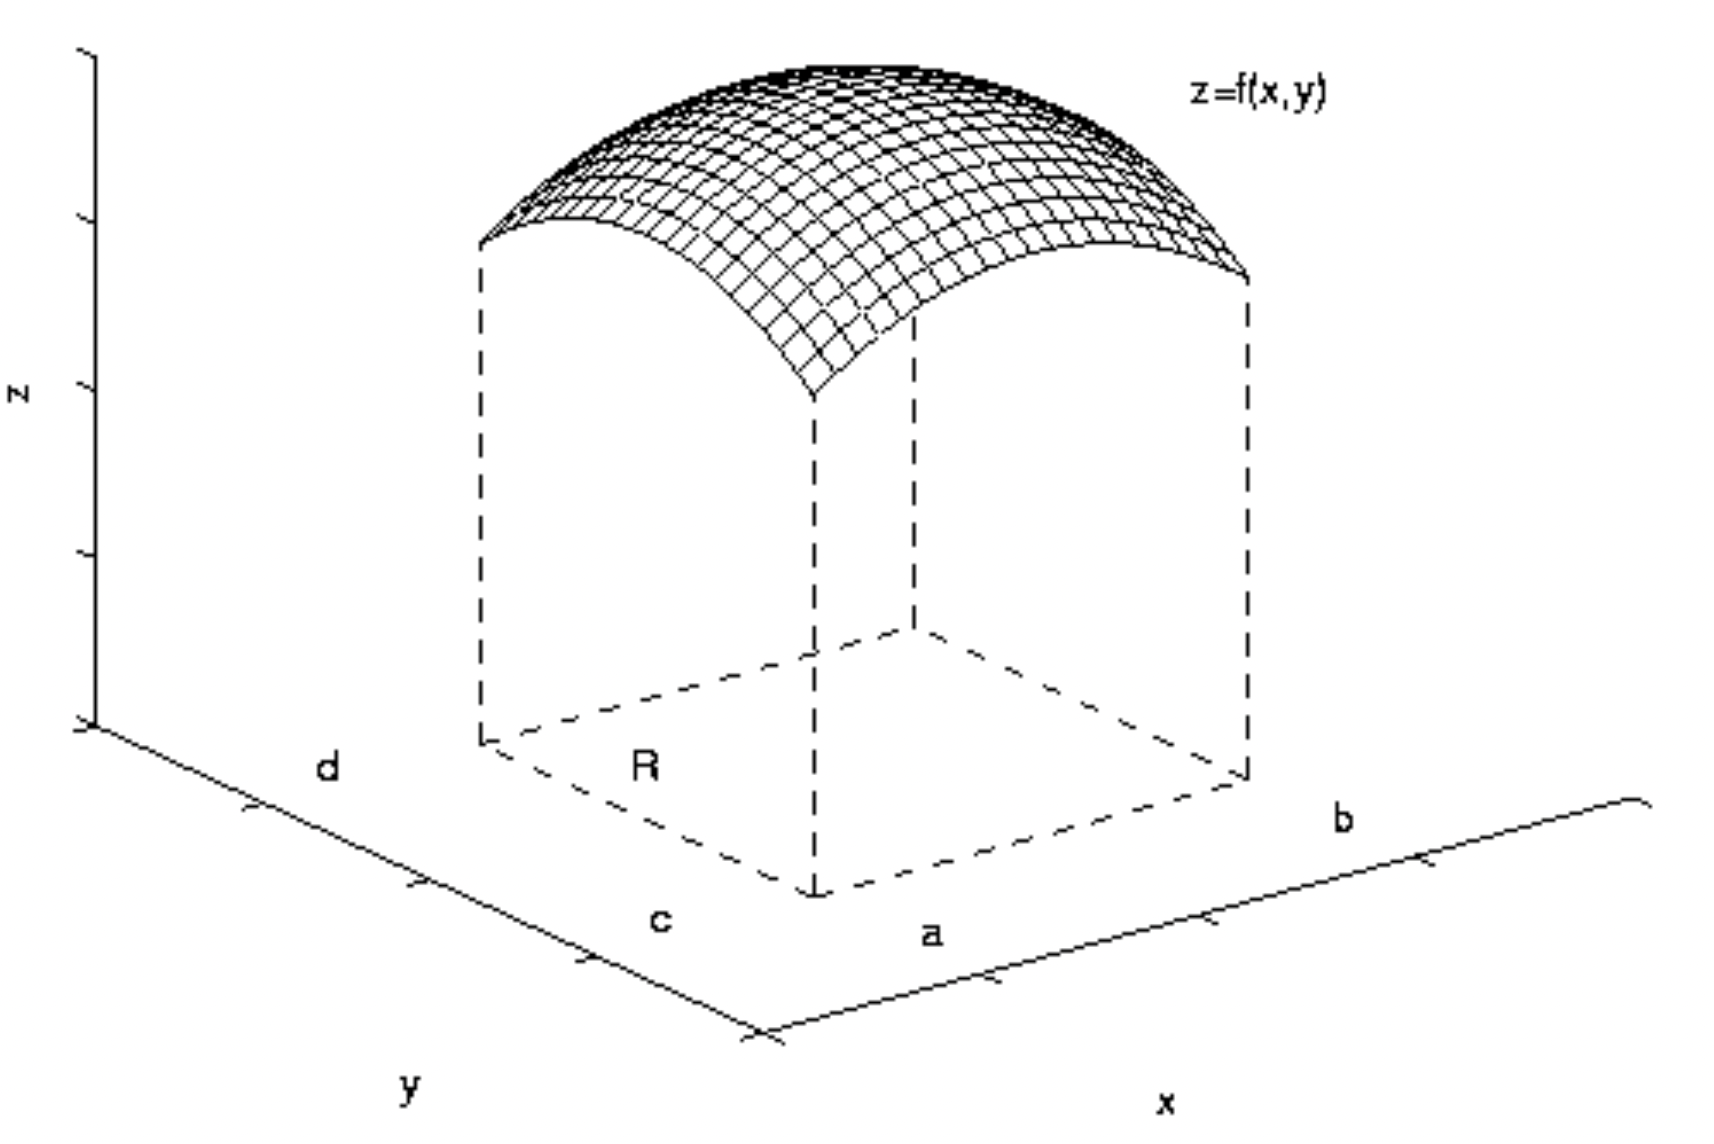
\includegraphics[width=0.75\linewidth]{Plots/s_4_1/Integral.png} \end{center}

In the above case, the domain is the rectangle on the $xy$-plane, with $x$ between $[a, b]$ and $y$ between $[c, d]$. For the volume, the base is always flat, but the top will usually be curved, since the function $z = f(x, y)$ tends to create a curved surface in 3D. If the domain had been a triangle, then the value of the integral would be the volume of a triangular prism, except the top will be curved.

Thus, when we try to integrate a 2D function $f(x, y)$ over any domain that is a 1D curve in the $xy$-plane, we would be trying to find the volume above the 1D curve. By agreeing that a curve is infinitely thin, we conclude that \itblue{the volume above the curve must be zero}. This is why our domain of integration for $f(x, y)$ \bred{must be a 2D area}.

\subsection*{Compute 2D Integrals}

A 2D integral typically will look like $$\iint_D f(x,y) = \int_D f(x, y) = \int_D f(x,y) \,dA$$ where $D$ is some 2D domain on the $xy$-plane.

To compute a 2D integral, we do not plot the function in 3D space. We split the 2D integral into 2 components, with $dx$ and $dy$.

\begin{enumerate}
    \item Draw the domain in the $xy$-plane.

    \item For all points inside the domain, determine the maximum and minimum values of $x$. These two values will be constant numbers $x_{min}$ and $x_{max}$.

    \item Pick a random value of $x$ between the minimum and maximum. Consider the vertical line that passes through the point $x$. Consider the maximum and minimum values of $y$ on the vertical line.

    \item Repeat step 3 several times. For different values of $x$ chosen, the max and min values of $y$ would be different. Typically, all the minimum values of $y$ would lie on a smooth curve, $y_{min} = m(x)$. Similarly, the maximum values would be the same, $y_{max} = M(x)$. In other words, the max and min of $y$ are \bred{functions of $x$}.

    \item Thus the integral can be evaluated as $$\int_D f(x, y) = \int_{x=x_{min}}^{x=x_{max}} \left( \int_{y=M(x)}^{y=m(x)} \,dy \right) \,dx$$ where the \bred{1D integral} inside the bracket is evaluated first. When carrying out integration with $dy$, we pretend that the variable $x$ is constant in the integration. We use the results of the inner integral, to carry out the integral outside the brackets with $dx$ afterwards.
\end{enumerate}

In the above steps, we first \bred{fix} $x$, and let $y$ vary between the lower bound curve and the upper bound curve while integrating. Then we add (integrate) all possible values of $x$.

We can also do the reverse by first attaining the min and max values of $y$ in the domain.

\begin{enumerate}
    \item Draw the domain in the $xy$-plane.

    \item For all points inside the domain, determine the maximum and minimum values of $y$. These two values will be constant numbers $y_{min}$ and $y_{max}$.

    \item Pick a random value of $y$ between the minimum and maximum. Consider the horizontal line that passes through the point $y$. Consider the maximum and minimum values of $x$ on the horizontal line. 

    \item Repeat step 3 several times. For different values of y chosen, the max and min values of x would be different. Typically, all the minimum values of x would lie on a smooth curve, xmin = m(y). Similarly, the maximum values would be the same, $x_{max} = M(y)$. In other words, the max and min of $x$ are \bred{functions of $y$}.

    \item Thus the integral can be evaluated as $$\int_D f(x, y) = \int_{y=y_{min}}^{y=y_{max}} \left( \int_{x=M(y)}^{x=m(y)} \,dx \right) \,dy$$ where the \bred{1D integral} inside the bracket is evaluated first. 
    
    Notice in the inner integral, $x$ is integrated first, and $y$ is regarded as constant. Here, $y$ is integrated after $x$, whereas in the previous way, $x$ is integrated after $y$. This is sometimes called \itblue{changing the order of integration}.

    This is not a good name since, when the order is changed, the limits of integrating are almost \bred{never the same}. In fact, the outer integral would always have limits that are constant numbers.
\end{enumerate}

Fubini's Theorem tells us that the 2 results will always be the same regardless of the order we choose, so we are free to choose the order of integration to our convenience when calculating 2D integrals \footnote{Fubini's Theorem requires all relevant integrals to be integrable. Typically no division by zero will ensure the function is integrable. }. 

Sometimes this may be used to our advantage, as some functions do not have 1D antiderivatives.

\subsection*{Properties of Integrals}

For integrals over some domain $D$ in $\mathbb{R}^n$ with integrable functions 

{~~~}

\begin{itemize}
    \item $\int_D(f + g) = \int_D f + \int_D g$ and $\int_D cf = c \int_D f$.
    
    \item If $f \le g$ on all of $D$, then $\int_D f \le \int_D g$. 
    
    \item $|f|$ is integrable if $f$ is integrable, and $\left| \int_D f \right| = \int_D |f|$. 

    \item If domain $C$ is contained in $D$ and $f \ge 0$, then $\int_C f \le \int_D f$. 
    
    \item For domain $C$ and $D$ (that we usually see), $\int_{C \cup D} f = \int_C f + \int_D f - \int_{C \cap D} f$. 
\end{itemize}

Notice that all properties of integral are shared with the integral in 1D.

\subsection*{Sharp Points on the Boundary of Domain}

In the case where the domain has a sharp point in the boundary, we can split up domain at the sharp point into 2 pieces, and integrate the 2 pieces separately, then add up the answers.

\subsection*{$n$-dimensional Volume}

For any set $D$ in $\mathbb{R}^n$, define the $n$-dimensional volume of $D$ $$V = \int_D 1$$ (Note: here $f = 1$, the constant function). 

\begin{itemize}
    \item If $n = 1$, then $V$ is the length of $D$ (1D interval with 1-dimensional volume). 
    \item If $n = 2$, then $V$ is the area of $D$ (2D area with 2-dimensional volume). 
    \item If $n = 3$, then $V$ is the volume of $D$ (3D volume with 3-dimensional volume). 
\end{itemize}

\begin{example}
    Let $f(x, y) = 10$. Let $D$ be the unit square between $0$ and $1$. 
    
    By noticing that the function is constant, we can see that the plot in 3D space will be a flat surface. The integral will represent the \bred{volume of the rectangular prism}, which can be calculated as base area $\times$ height. Thus, the answer will be $10 \cdot 1 = 10$.

    We can also evaluate the integral using the above steps.

    Drawing the domain, we see that the min and max values of $x$ is $0$ and $1$. For any fixed value of $x$, we see that the min and max values of $y$ is $0$ and $1$.

    % TODO: finish the graph
    \begin{center}
        \begin{tikzpicture}
                \draw[->] (-0.7, 0) -- (1.7, 0) node[right] {$x$};
                \draw[->] (0, -0.7) -- (0, 1.7) node[above] {$y$};

                \draw[DarkGreen] (0,0) rectangle (1,1);
        \end{tikzpicture}
    \end{center}
    \begin{align*}
        \int_D f(x,y)   = \int_D 10
                        = 10 \cdot \left( \int_D 1 \right)
                        = 10 \cdot \int_{x=0}^{x=1} \left( \int_{y=0}^{y=1} 1 \,dy \right) \,dx
                      & = 10 \cdot \int_{x=0}^{x=1} 1 \,dx                                      \\
                      & = 10
    \end{align*}
\end{example}

\begin{example}
    Let $f(x, y) = x$. Let $D$ be the triangle with vertices $(0, 0)$, $(1, 0)$, $(1, 2)$.

    Drawing the domain, The min and max values of $x$ is $0$ and $1$. For any fixed value of $x$, the min value of $y$ is $0$.

    However, the max value of $y$ changes. The max value of $y$ all lie on the curve $y = 2x = M(x)$.
    
    % TODO: finish the graph
    \begin{center}
        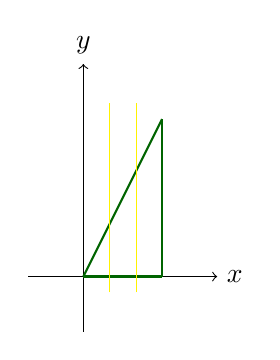
\begin{tikzpicture}
                \draw[->] (-0.7, 0) -- (1.7, 0) node[right] {$x$};
                \draw[->] (0, -0.7) -- (0, 2.7) node[above] {$y$};

                \draw[thick,DarkGreen] (0,0) -- (1,0);
                \draw[thick,DarkGreen] (1,0) -- (1,2);
                \draw[thick,DarkGreen] (1,2) -- (0,0);

                \draw[yellow] (0.33,-0.2) -- (0.33,2.2);
                \draw[yellow] (0.67,-0.2) -- (0.67,2.2);
        \end{tikzpicture}
    \end{center}
    \begin{align*}
        \int_D f(x,y)   = \int_D x
                        = \int_{x=0}^{x=1} \left( \int_{y=0}^{{\color{red}y=2x}} x \,dy \right) \,dx
                      & = \int_{x=0}^{x=1} x \left( \int_{y=0}^{{\color{red}y=2x}} 1 \,dy \right) \,dx \\
                      & = \int_{x=0}^{x=1} x \left( y \bigg|_{y=0}^{{\color{red}y=2x}} \right) \,dx    \\
                      & = \int_{x=0}^{x=1} x \cdot 2x \,dx                                             \\
                      & = \int_{x=0}^{x=1} 2x^2
                        = \frac{2}{3} x^3 \bigg|_{x=0}^{x=1}
                        = \frac{2}{3}
    \end{align*}

    Notice that the bound inside the inner integral is a function of $x$. Since we are integrating with $dy$, we regard $x$ as constant, and move it out of the integral.
\end{example}

\subsection*{Domain Defined Using Inequalities}

When domains are defined using an inequality, we take the inequality and make it equality. This will create a curve in the $xy$-plane which we can draw. We start on the curve, and move a little bit to the right of the curve. This increased the value of $x$, so one side of the equality has become larger. Using this information, we can determine the area defined by the equality.

\begin{example}
    Let $f(x, y)$ be a function. Let $D$ be bounded by $y = x$ and $y = x^2$.

    \begin{center}
        \tikzsetnextfilename{c04s01-f03}%
        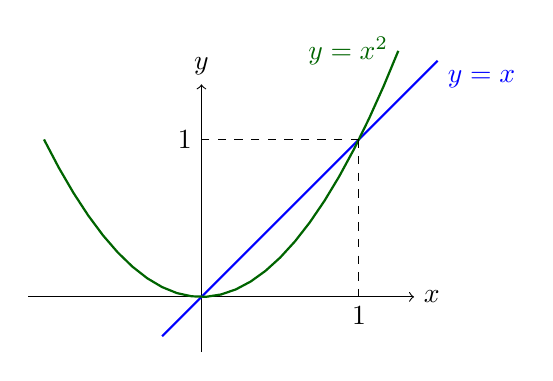
\begin{tikzpicture}
            \draw[->] (-2.2,0) -- (2.7,0) node[right] {$x$};
            \draw[->] (0,-0.7) -- (0,2.7) node[above] {$y$};

            \draw[thick,blue,domain=-0.5:3] plot (\x, {\x}) node[below right] {$y=x$};
            \draw[thick,DarkGreen,domain=-2:2.5] plot (\x, {((\x)^2)/2}) node[left] {$y=x^2$};

            \draw[dashed] (2,2) -- (2,0) node[below] {$1$};
            \draw[dashed] (2,2) -- (0,2) node[left] {$1$};
        \end{tikzpicture}
    \end{center}

    After drawing the curve, we see that the intersection is at $(0, 0)$ and $(1, 1)$. We see that the min value of $y$ lies on the curve $y = x^2 = m(x)$. The max value of $y$ is $y = x = M(x)$.
    $$\int_D f(x, y) = \int_{x=0}^{x=1} \left( \int_{y=x^2}^{y=x} f(x, y) \,dx \right) \,dy$$
\end{example}

\begin{example}
    Let $D$ be bounded by $y = x$ and $y = -x + 2$, $y = 0$.

    The max value of $y$ is not a smooth curve due to the sharp point at $x = 1$. We can split the integral in 2 pieces, with $x \in [0, 1]$, and $x \in [1, 2]$.
    $$\int_D f(x, y) = \int_{x=0}^{x=1} \left( \int_{y=0}^{y=x} f(x, y) \,dy \right) + \int_{x=1}^{x=2} \left( \int_{y=0}^{y=-x+2} f(x, y) \,dy \right)$$

    We can also interchange the order of integration.
\end{example}

\begin{exercise}
    Let $D$ be bounded by $y = x$ and $y = -x + 2$, $y = 0$.

    Compute the integral by changing the order of integration. Compare with example 4.4, notice that we no longer need to split up the domain, because the sharp point is now the endpoint of the integral.
\end{exercise}

\begin{exercise}
    Integrate $\int_D f(x, y)$. 

    \begin{enumerate}
        \item Let $D$ be bounded by $x = 0$, $y = 0$, $y = -2x + 2$. 
        \item Let $D$ be bounded by $y = x + 1$, $y = -x^2 + 1$.
        \item Let $D$ be the triangle defined by $(0, 2)$, $(0, -2)$, $(2, 0)$.
        \item Let $D = \{ (x, y) \in \mathbb{R}^2 | x \in [0, 1], y \in [0, 1], y > x^2 \}$
    \end{enumerate}
\end{exercise}

\begin{exercise}
    Evaluate $$\int_{y=0}^{y=1} \left( \int_{x=0}^{x=y^4} y \frac{\sin{x}}{(1 - \sqrt{x})} \,dx \right) \,dy$$

    \textbf{Strategy:}

    The function looks difficult. What is the region of integration? Try changing the order of integration.
\end{exercise}

\begin{exercise}
    Evaluate

    {~~~}

    \begin{enumerate}
        \item $\int_{x=0}^{x=8} \left( \int_{y=\sqrt[3]{x}}^{y=2} \frac{x}{y^7 +1} \,dy \right) \,dx$
        \item $\int_{x=0}^{x=4} \left( \int_{y=\sqrt{x}}^{y=2} y \cos(y^4 + 3) \,dy \right) \,dx$
        \item $\int_{y=0}^{y=1} \left( \int_{x=y}^{x=\sqrt{y}} \frac{\sin{x}}{x} \,dx \right) \,dy$
        \item $\int_{y=0}^{y=1} \left( \int_{x=0}^{x=arccos{y}} e^{2\sin{x}} \,dx \right) \,dy$
    \end{enumerate}
\end{exercise}

\section{Regular Integral in 3D}

To compute integral of $f(x,y,z)$ over a 3 dimensional domain $D$, it is similar.

\begin{enumerate}
    \item Draw the domain in 3D. (This is difficult). 

    \item Take the \bred{projection} of the 3D domain onto one of the 3 planes created by the axis. This creates a 2D domain. Suppose in this case, we take the projection onto the $xy$-plane.
    
    \item Compute the limits of integration for the 2D domain in $xy$-plane (as a 2D integral). These will be the limits of the outer most integrals. Match $dx$ and dy according to the order used. 
    
    \item Pick a random point $(x, y)$ in the projection. Consider the \bred{vertical} line in the $z$ direction. Consider the maximum and minimum values of $z$. 
    
    \item Repeat step $4$ several times. The min and max values of $z$ usually will be on a smooth surface that depend on the point $(x, y)$. Thus $z_{min} = m(x, y)$ and $z_{max} = M(x, y)$.
    
    These are the limits of the inner most integral, with $dz$.
    $$\int_D f(x, y, z) = \int_{2D} \left( \int_{z=m(x,y)}^{z=M(x,y)} f(x, y, z) \,dz \right) \,dx \,dy$$
    where the order of $dx \,dy$ depends upon the order chosen for the 2D integral. In general, inner limits can depend on variables from outer integrals, but limits of outer integrals never depend on variables from inner integrals. 
\end{enumerate}

When an equation involves only 2 variables (in 3D), it gives a curve in 2D which extends infinitely toward the 3rd dimension, giving a cylinder-like surface in 3D. With 2 such curves, we will get at least 2 intersection points. Connecting the intersection points with a ``smooth'' curve typically gives the picture of the domain in 3D.

\begin{exercise}
    Let $D$ be bounded by the given equations, in first octant. 

    Compute the integral $\int_D f(x, y, z)$ in 6 ways (3 ways to project, 2 ways to compute the 2D integral of the projection). 

    \begin{minipage}[t]{0.45\linewidth}
        \begin{enumerate}
            \item $z = 1 - x$, $y = 1$
            \item $z = 1 - y$, $x = y^2$
            \item $z = 1 - x^2$, $y = 1 - x$
        \end{enumerate}
    \end{minipage}
    \begin{minipage}[t]{0.45\linewidth}
        \begin{enumerate} \setcounter{enumi}{3}
            \item $z = 1 - y^2$, $y = x$
            \item $y^2 + z^2 = 9$, $y = 3x$
            \item $2x + y + 2z = 1$
        \end{enumerate}
    \end{minipage}
\end{exercise}